\chapter{問題意識}
本章では,本研究における問題意識を洗い出す.
はじめに筆者が本研究に先立ち行った研究について説明し,ついで前章での関連研究も含めた問題意識について述べる.

\section{他ユーザの記録表示を通じた学習の動機づけ向上}
本研究に先立ち,学習記録アプリケーション``Stuguin"にて他者の記録を表示することにより動機づけの向上を図った研究を行った~\cite{hashiba}.
Stuguinシステムの詳細については次章以降で述べる.
この評価実験では,被験者を表~\ref{tb:pre_group}のように4群に分け,各群において他者の記録の選出基準を変えた.
{\bf More}群,{\bf Same}群,{\bf Less}群の学習記録選出の条件を図~\ref{fig:election}に,実際に他ユーザの記録を表示した画面を図~\ref{fig:recent_records}に示す.

\begin{table}[htb]
\begin{center}
  \begin{tabular}{|l|l|l|} \hline
    グループ & 選出基準 & 人数 \\ \hline
	{\bf More}群 & 自身の学習時間よりも多い記録を選出する & 6名 \\
    {\bf Same}群 & 自身と同程度の記録を選出する & 9名 \\
    {\bf Less}群 & 自身の学習時間よりも少ない記録を選出する & 5名 \\ 
	{\bf Random}群 & ランダムに選出する & 6名 \\
	{\bf None}群 & 他ユーザの記録を表示しない & 12名 \\ \hline
  \end{tabular}
  \caption{被験者グループ}
  \label{tb:pre_group}
\end{center}
\end{table}

\begin{figure}[htb]
	\begin{center}
	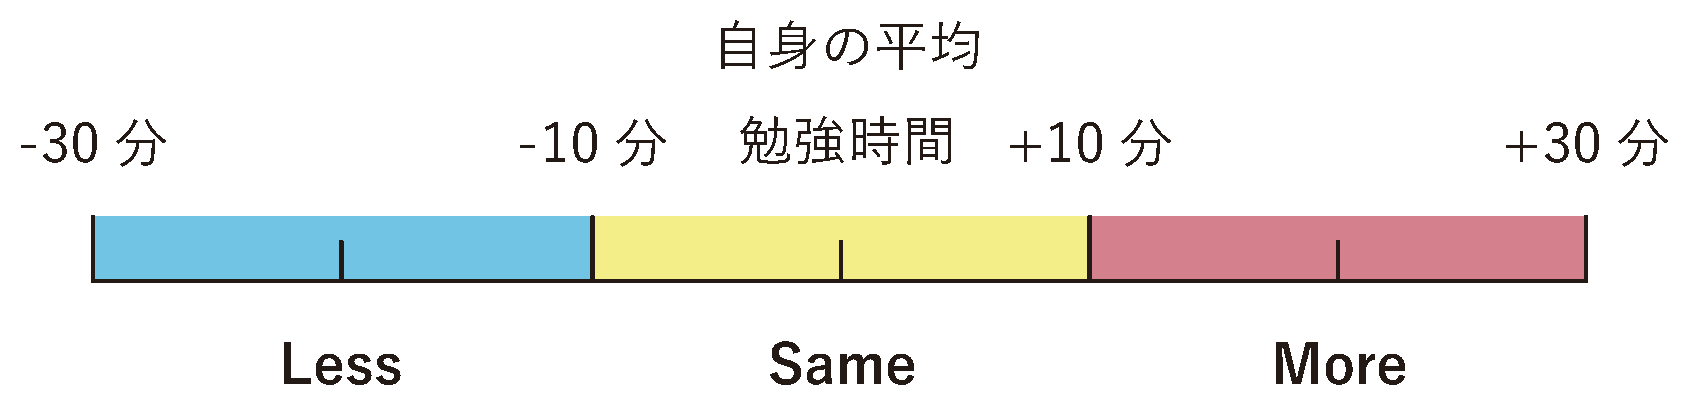
\includegraphics[width=9cm]{images/3/election.eps}
	\end{center}
	\caption{選出基準}
	\label{fig:election}
\end{figure}

\begin{figure}[htb]
	\begin{center}
	\includegraphics[width=5cm]{images/3/recent_records.eps}
	\end{center}
	\caption{他ユーザの学習記録表示}
	\label{fig:recent_records}
\end{figure}

ユーザ38名に対して行った8週間の評価実験では,前半4週間は全被験者に対して他ユーザの記録を表示せず,後半4週間にてグループごとに表示を変えた.
5群の中で,自身の学習時間よりも多い記録を選出した{\bf More}群の平均学習時間,学習記録回数が共に増加した.
グループごとの1記録における平均学習時間を図~\ref{fig:average_study_time}に,平均学習記録回数を図~\ref{fig:average_of_study_session}に示す.

\begin{figure}[ht]
\begin{center}
\begin{tabular}{c}

	\begin{minipage}[b]{0.5\linewidth}
	\begin{center}
		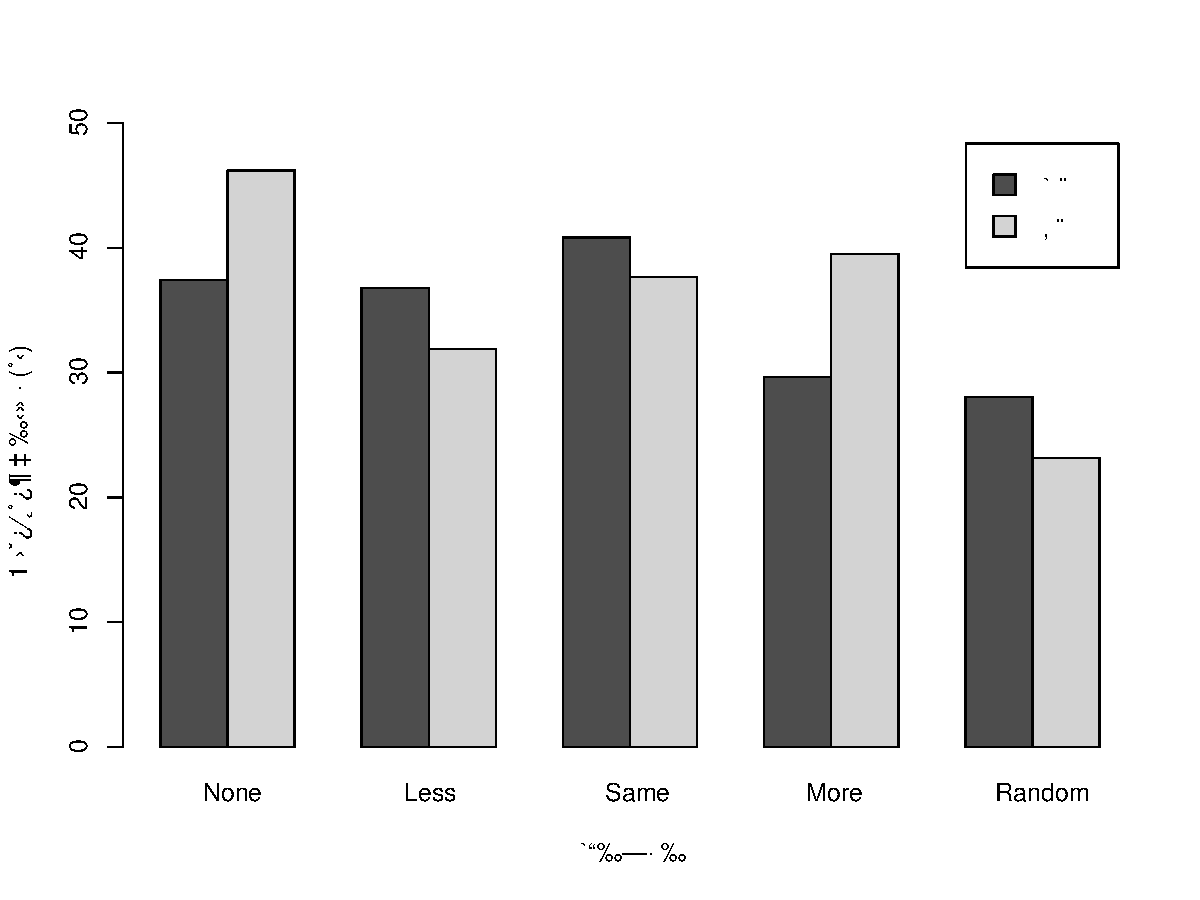
\includegraphics[width=8cm]{images/3/average_of_studying_time.pdf}
		\caption{1記録の平均学習時間}
		\label{fig:average_study_time}
	\end{center}
	\end{minipage}

	\begin{minipage}[b]{0.5\linewidth}
	\begin{center}
		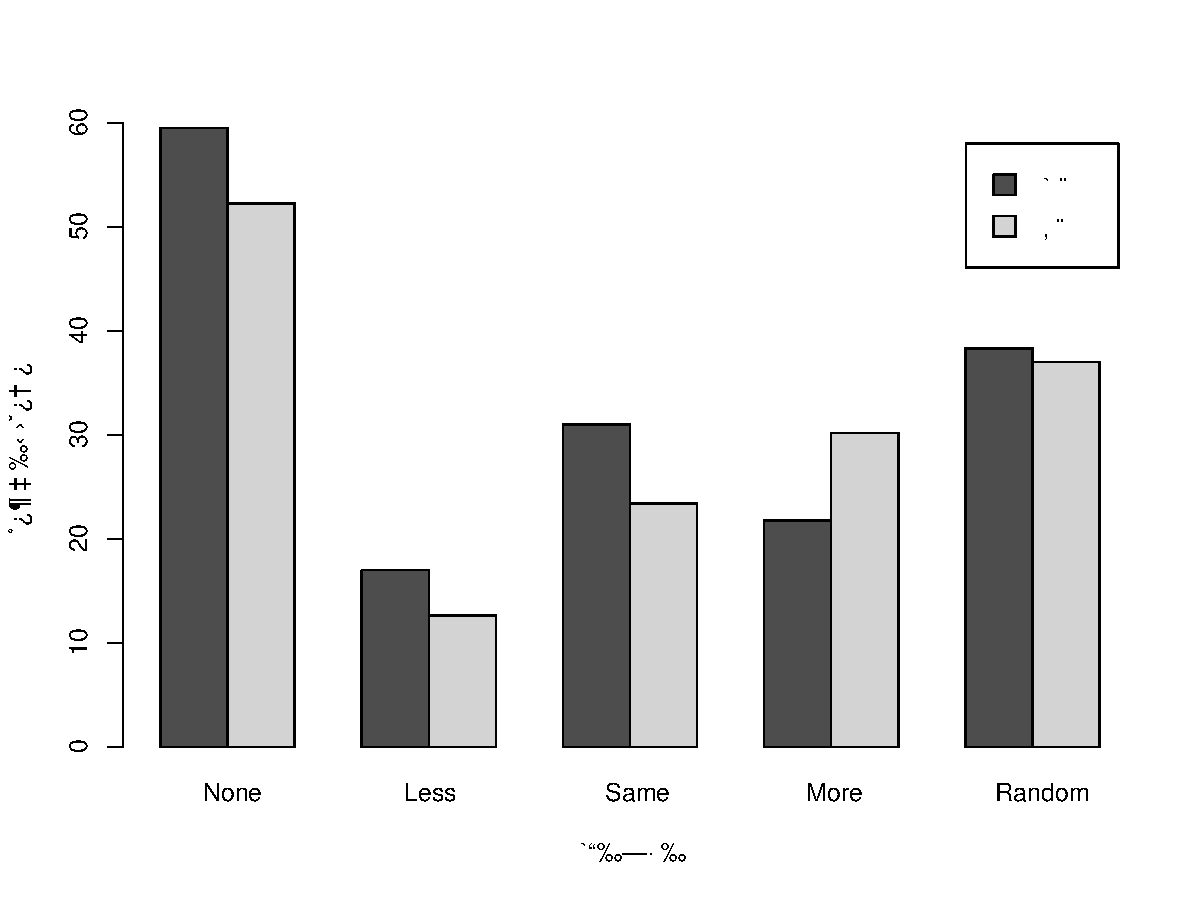
\includegraphics[width=8cm]{images/3/average_of_study_session.pdf}
		\caption{平均学習記録回数}
		\label{fig:average_of_study_session}
	\end{center}
	\end{minipage}

\end{tabular}
\end{center}
\end{figure}

これより,他者の記録表示が学習への動機づけの向上に有効である可能性が示された.

{\bf None}群においては,日数が経つにつれどの被験者も学習時間が低下することを予想していたが,両期間を通して高い動機づけを維持した被験者も確認できた.
反対に他者比較を行ったグループにおいて,学習時間や記録頻度が著しく低下した被験者も存在した.
同じグループ内でも動機づけ向上に対する効果に違いが見られたのは,各被験者が学習に対して異なる動機づけ状態であったことが考えられる.

\section{学習者が抱く動機づけタイプの未検討}
基本的には,外的な動機づけ要因は動機づけの内在化を妨げ,パフォーマンスを下げる.
Mollerら~\cite{moller2006self}の研究では,内的に動機づけられた行動に対して金銭報酬を与えた際,その動機づけが阻害されるというアンダーマイニング効果について述べられている.
また,冷水ら~\cite{shimizu}による研究では,金銭報酬群と他者比較群に分けて運動課題を与えたところ,他者比較群に優位な学習効果が見られた.
より内的な要因による動機づけの方が,学習のパフォーマンスや成績においても優れたものとなることがわかる.

一方で,たとえ外発的に動機づけられた行動であっても,その行動に対する個人の価値の認め方によっては,自己決定性は高くなる~\cite{ryan2000self}.
例えば,外的調整による動機づけを抱く学習者にとっては,罰や報酬の存在は,学習を行うことの自己決定性を高める要因となる.
結果として,内発的動機づけに近い形で学習成績やパフォーマンス,精神的健康に良好な影響を及ぼす.
つまり,学習者抱く動機づけに応じたアプローチを行うことが,動機づけの向上及び内在化に有用な方策として考えられる.

しかしながら既存研究では,筆者が行った研究も含め,被験者らが持つ動機づけの種類を考慮していない.
学習者はそれぞれ異なる動機づけを抱いており,その動機づけに適した外部刺激を与えることで動機づけの向上及び内在化を促すことができる.
したがって本研究では,学習者の抱く動機づけタイプに応じてアプローチを切り替えることで,学習に対する動機づけの向上及び内在化を図る.

\section{まとめ}
本章では,筆者が本研究に先立ち行った研究について述べ,問題意識を洗い出した.
次章では,本論文において提案するシステムの要件について述べる.